\documentclass[tikz,border=10pt]{standalone}
\usepackage{tikz}
\usetikzlibrary{shapes.geometric}

\begin{document}
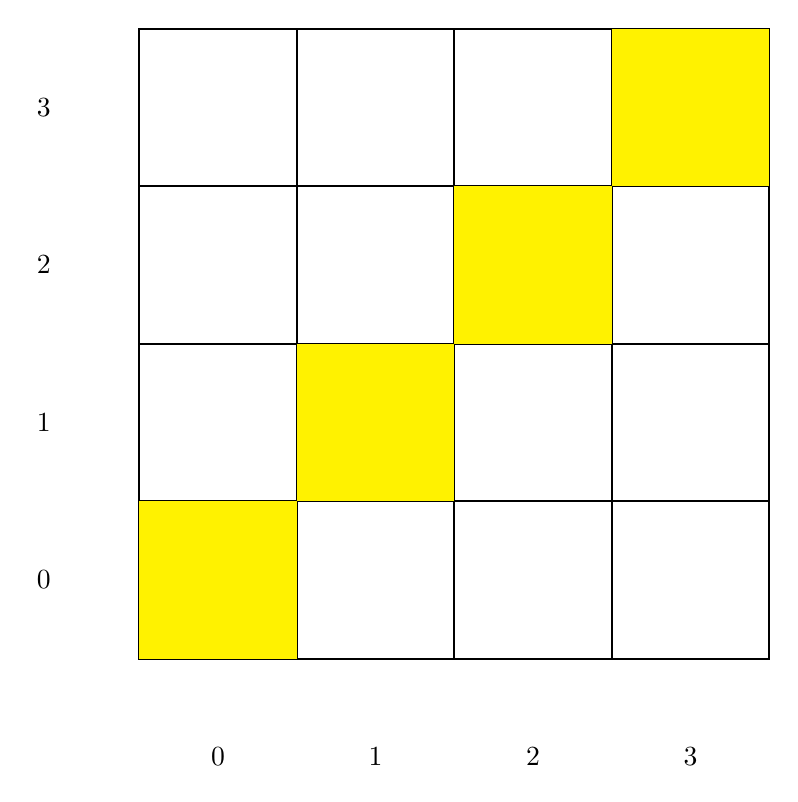
\begin{tikzpicture}[scale=2]
    % Draw the 4x4 grid
    \foreach \x in {0,1,2,3} {
        \foreach \y in {0,1,2,3} {
            \draw[thick] (\x,\y) rectangle ++(1,1);
        }
    }

    % Mark active antennas in yellow
    \fill[yellow] (0,0) rectangle ++(1,1); % Top-left
    \fill[yellow] (1,1) rectangle ++(1,1); % Center-right
    \fill[yellow] (2,2) rectangle ++(1,1); % Bottom-left
    \fill[yellow] (3,3) rectangle ++(1,1); % Bottom-right

    % Add labels for clarity
    \node at (0.5,-0.5) [below] {0};
    \node at (1.5,-0.5) [below] {1};
    \node at (2.5,-0.5) [below] {2};
    \node at (3.5,-0.5) [below] {3};

    \node at (-0.5,0.5) [left] {0};
    \node at (-0.5,1.5) [left] {1};
    \node at (-0.5,2.5) [left] {2};
    \node at (-0.5,3.5) [left] {3};

\end{tikzpicture}
\end{document}